\documentclass[
  shownotes,
  xcolor={svgnames},
  hyperref={colorlinks,citecolor=DarkBlue,linkcolor=DarkRed,urlcolor=DarkBlue}
  , aspectratio=169]{beamer}
\usepackage{animate}
\usepackage{amsmath}
\usepackage{amsfonts}
\usepackage{amssymb}
\usepackage{pifont}
\usepackage{mathpazo}
%\usepackage{xcolor}
\usepackage{multimedia}
\usepackage{fancybox}
\usepackage[para]{threeparttable}
\usepackage{multirow}
\setcounter{MaxMatrixCols}{30}
\usepackage{subcaption}
\usepackage{graphicx}
\usepackage{lscape}
\usepackage[compatibility=false,font=small]{caption}
\usepackage{booktabs}
\usepackage{ragged2e}
\usepackage{chronosys}
\usepackage{appendixnumberbeamer}
\usepackage{animate}
\setbeamertemplate{caption}[numbered]
\usepackage{color}
%\usepackage{times}
\usepackage{tikz}
\usepackage{comment} %to comment
%% BibTeX settings
\usepackage{natbib}
\bibliographystyle{apalike}
\bibpunct{(}{)}{,}{a}{,}{,}
\setbeamertemplate{bibliography item}{[\theenumiv]}

% Defines columns for bespoke tables
\usepackage{array}
\newcolumntype{L}[1]{>{\raggedright\let\newline\\\arraybackslash\hspace{0pt}}m{#1}}
\newcolumntype{C}[1]{>{\centering\let\newline\\\arraybackslash\hspace{0pt}}m{#1}}
\newcolumntype{R}[1]{>{\raggedleft\let\newline\\\arraybackslash\hspace{0pt}}m{#1}}


\usepackage{xfrac}


\usepackage{multicol}
\setlength{\columnsep}{0.5cm}

% Theme and colors
\usetheme{Boadilla}

% I use steel blue and a custom color palette. This defines it.
\definecolor{andesred}{HTML}{af2433}

% Other options
\providecommand{\U}[1]{\protect\rule{.1in}{.1in}}
\usefonttheme{serif}
\setbeamertemplate{itemize items}[default]
\setbeamertemplate{enumerate items}[square]
\setbeamertemplate{section in toc}[circle]

\makeatletter

\definecolor{mybackground}{HTML}{82CAFA}
\definecolor{myforeground}{HTML}{0000A0}

\setbeamercolor{normal text}{fg=black,bg=white}
\setbeamercolor{alerted text}{fg=red}
\setbeamercolor{example text}{fg=black}

\setbeamercolor{background canvas}{fg=myforeground, bg=white}
\setbeamercolor{background}{fg=myforeground, bg=mybackground}

\setbeamercolor{palette primary}{fg=black, bg=gray!30!white}
\setbeamercolor{palette secondary}{fg=black, bg=gray!20!white}
\setbeamercolor{palette tertiary}{fg=white, bg=andesred}

\setbeamercolor{frametitle}{fg=andesred}
\setbeamercolor{title}{fg=andesred}
\setbeamercolor{block title}{fg=andesred}
\setbeamercolor{itemize item}{fg=andesred}
\setbeamercolor{itemize subitem}{fg=andesred}
\setbeamercolor{itemize subsubitem}{fg=andesred}
\setbeamercolor{enumerate item}{fg=andesred}
\setbeamercolor{item projected}{bg=gray!30!white,fg=andesred}
\setbeamercolor{enumerate subitem}{fg=andesred}
\setbeamercolor{section number projected}{bg=gray!30!white,fg=andesred}
\setbeamercolor{section in toc}{fg=andesred}
\setbeamercolor{caption name}{fg=andesred}
\setbeamercolor{button}{bg=gray!30!white,fg=andesred}


\usepackage{fancyvrb}
\newcommand{\VerbBar}{|}
\newcommand{\VERB}{\Verb[commandchars=\\\{\}]}
\DefineVerbatimEnvironment{Highlighting}{Verbatim}{commandchars=\\\{\}}
% Add ',fontsize=\small' for more characters per line
\usepackage{framed}
\definecolor{shadecolor}{RGB}{248,248,248}
\newenvironment{Shaded}{\begin{snugshade}}{\end{snugshade}}
\newcommand{\AlertTok}[1]{\textcolor[rgb]{0.94,0.16,0.16}{#1}}
\newcommand{\AnnotationTok}[1]{\textcolor[rgb]{0.56,0.35,0.01}{\textbf{\textit{#1}}}}
\newcommand{\AttributeTok}[1]{\textcolor[rgb]{0.77,0.63,0.00}{#1}}
\newcommand{\BaseNTok}[1]{\textcolor[rgb]{0.00,0.00,0.81}{#1}}
\newcommand{\BuiltInTok}[1]{#1}
\newcommand{\CharTok}[1]{\textcolor[rgb]{0.31,0.60,0.02}{#1}}
\newcommand{\CommentTok}[1]{\textcolor[rgb]{0.56,0.35,0.01}{\textit{#1}}}
\newcommand{\CommentVarTok}[1]{\textcolor[rgb]{0.56,0.35,0.01}{\textbf{\textit{#1}}}}
\newcommand{\ConstantTok}[1]{\textcolor[rgb]{0.00,0.00,0.00}{#1}}
\newcommand{\ControlFlowTok}[1]{\textcolor[rgb]{0.13,0.29,0.53}{\textbf{#1}}}
\newcommand{\DataTypeTok}[1]{\textcolor[rgb]{0.13,0.29,0.53}{#1}}
\newcommand{\DecValTok}[1]{\textcolor[rgb]{0.00,0.00,0.81}{#1}}
\newcommand{\DocumentationTok}[1]{\textcolor[rgb]{0.56,0.35,0.01}{\textbf{\textit{#1}}}}
\newcommand{\ErrorTok}[1]{\textcolor[rgb]{0.64,0.00,0.00}{\textbf{#1}}}
\newcommand{\ExtensionTok}[1]{#1}
\newcommand{\FloatTok}[1]{\textcolor[rgb]{0.00,0.00,0.81}{#1}}
\newcommand{\FunctionTok}[1]{\textcolor[rgb]{0.00,0.00,0.00}{#1}}
\newcommand{\ImportTok}[1]{#1}
\newcommand{\InformationTok}[1]{\textcolor[rgb]{0.56,0.35,0.01}{\textbf{\textit{#1}}}}
\newcommand{\KeywordTok}[1]{\textcolor[rgb]{0.13,0.29,0.53}{\textbf{#1}}}
\newcommand{\NormalTok}[1]{#1}
\newcommand{\OperatorTok}[1]{\textcolor[rgb]{0.81,0.36,0.00}{\textbf{#1}}}
\newcommand{\OtherTok}[1]{\textcolor[rgb]{0.56,0.35,0.01}{#1}}
\newcommand{\PreprocessorTok}[1]{\textcolor[rgb]{0.56,0.35,0.01}{\textit{#1}}}
\newcommand{\RegionMarkerTok}[1]{#1}
\newcommand{\SpecialCharTok}[1]{\textcolor[rgb]{0.00,0.00,0.00}{#1}}
\newcommand{\SpecialStringTok}[1]{\textcolor[rgb]{0.31,0.60,0.02}{#1}}
\newcommand{\StringTok}[1]{\textcolor[rgb]{0.31,0.60,0.02}{#1}}
\newcommand{\VariableTok}[1]{\textcolor[rgb]{0.00,0.00,0.00}{#1}}
\newcommand{\VerbatimStringTok}[1]{\textcolor[rgb]{0.31,0.60,0.02}{#1}}
\newcommand{\WarningTok}[1]{\textcolor[rgb]{0.56,0.35,0.01}{\textbf{\textit{#1}}}}
\usepackage{graphicx}
\makeatletter

\definecolor{airforceblue}{rgb}{0.36, 0.54, 0.66}

\usepackage{tikz}
% Tikz settings optimized for causal graphs.
\usetikzlibrary{shapes,decorations,arrows,calc,arrows.meta,fit,positioning}
\tikzset{
    -Latex,auto,node distance =1 cm and 1 cm,semithick,
    state/.style ={ellipse, draw, minimum width = 0.7 cm},
    point/.style = {circle, draw, inner sep=0.04cm,fill,node contents={}},
    bidirected/.style={Latex-Latex,dashed},
    el/.style = {inner sep=2pt, align=left, sloped}
}


\makeatother






%%%%%%%%%%%%%%% BEGINS DOCUMENT %%%%%%%%%%%%%%%%%%

\begin{document}
 
\title[Lecture 25]{Lecture 25:  Boosting and Gradients}
\subtitle{Big Data and Machine Learning for Applied Economics \\ Econ 4676}
\date{\today}

\author[Sarmiento-Barbieri]{Ignacio Sarmiento-Barbieri}
\institute[Uniandes]{Universidad de los Andes}


\begin{frame}[noframenumbering]
\maketitle
\end{frame}

%%%%%%%%%%%%%%%%%%%%%%%%%%%%%%%%%%%





%----------------------------------------------------------------------%
\section{Announcements}
%----------------------------------------------------------------------%
\begin{frame}
\frametitle{Announcements}

\begin{itemize}
\item Problem Set 4: Next Friday presentations
\medskip
\item Thursday you need to submit a .csv it at 8:00 pm. 
  \begin{itemize}
    \item Please upload it to your repo don't forget to follow the instructions, if you have questions ask before hand, {\bf not at 7:30pm before submission!} 
    \medskip
    \item The lowest the better the score (smaller loss)
    \medskip
    \item If you forget to send me the number of parameters I'll assign $100,000$
    \medskip
    \item If I can't grab you predictions file from your repo with  \texttt{grep} you won't get credit for the problem set.
  \end{itemize}
\medskip
\item I've uploaded the final presentation schedule
\end{itemize}

\end{frame}
%----------------------------------------------------------------------% 

\begin{frame}
\frametitle{Announcements}

\begin{itemize}

  \item I've uploaded the final presentation schedule
    \medskip
  \item Presentations will be in the following order:

  \begin{itemize}
    \item November 30th
    \begin{enumerate}
        \item Bares y Rendimiento Educativo (Arrieta y Montero)
        \item Startup Failure (Rodriguez)
        \item Covid-19 (Saenz)
        \item Precios Propiedades (Gonzalez)
      \end{enumerate}
      \item December 2nd
      \begin{enumerate}
        \item Cambio Estructural (Rengifo)
        \item Booktopia (Agudelo, Cepeda, Cifuentes, y Mosquera)
        \item Rendimiento Educativo (Salazar, Cortes, Rojas, y Peña)
        \end{enumerate}
        \item December 3rd
        \begin{enumerate}
          \item Pobreza Multidimensional (Miranda)
          \item Demanda de Energía (Ramírez y Castro)
          \item Basketball (Segura, Prieto y Navarro)
        \end{enumerate}
  \end{itemize}
    \end{itemize}

\end{frame}
%----------------------------------------------------------------------% 

\begin{frame}
\frametitle{Agenda}

\tableofcontents

\end{frame}

%----------------------------------------------------------------------%
\section{Recap: Trees, Forests, and Boosting}
%----------------------------------------------------------------------%
\begin{frame}[fragile]
\frametitle{ Trees }

\begin{figure}[H] \centering
            \captionsetup{justification=centering}
              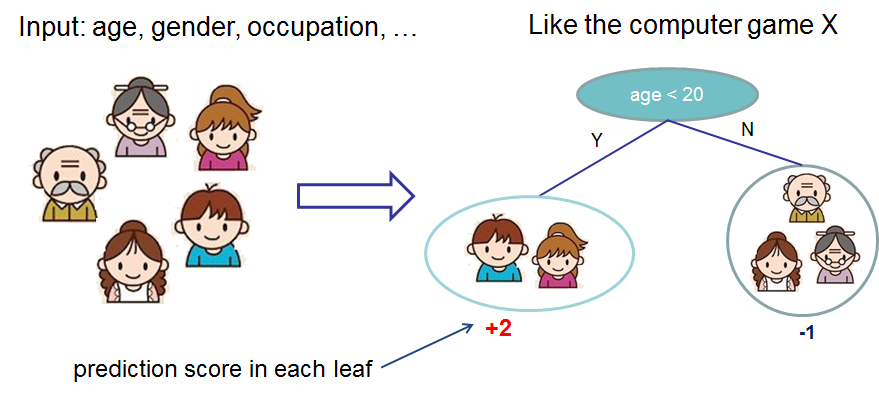
\includegraphics[scale=0.5]{figures/cart}
              \\
              \tiny
              \url{source: https://xgboost.readthedocs.io/en/latest/tutorials/model.html}
 \end{figure}



\end{frame}
%----------------------------------------------------------------------%
\begin{frame}[fragile]
\frametitle{ Forests }


\begin{itemize}
  \item We can improve performance a lot using either bootstrap aggregation (bagging), random forests, or boosting.
  \item Bagging \& Random Forests:
    \begin{itemize}
      \item Repeatedly draw bootstrap samples $(X_i^b,Y_i^b)_{i=1}^N$ from the observed sample.
      \item For each bootstrap sample, fit a regression tree $\hat{f}^b(x)$
      \begin{itemize}
        \item Bagging: full sample
        \item Random Forests: subset of predictors $ \sqrt(p)$ (breaks high correlation)
      \end{itemize}
      \item Average across bootstrap samples to get the predictor
      \begin{align}
        \hat{f}_{bag} =\frac{1}{B}\sum_{b=1}^B \hat{f}^b(x)
      \end{align}
\item Basically we are smoothing predictions. 
\item Idea: the variance of the average is less than that of a single prediction.
\end{itemize}

\end{itemize}


\end{frame}
%----------------------------------------------------------------------%
\begin{frame}[fragile]
\frametitle{ Forests }

\begin{figure}[H] \centering
            \captionsetup{justification=centering}
              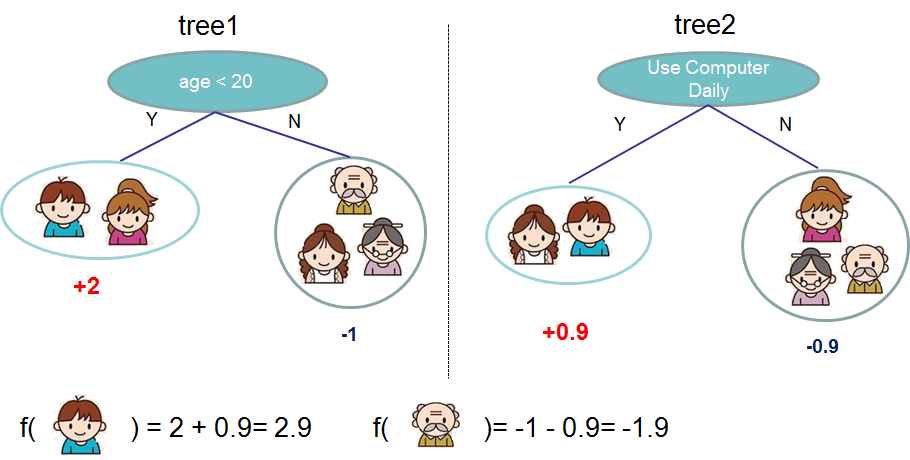
\includegraphics[scale=0.5]{figures/twocart.png}
              \\
              \tiny
              \url{source: https://xgboost.readthedocs.io/en/latest/tutorials/model.html}
 \end{figure}



\end{frame}
%----------------------------------------------------------------------%
\section{Boosting}
\subsection{Motivation}
%----------------------------------------------------------------------%
\begin{frame}[fragile]
\frametitle{Boosting: Motivation}

\begin{itemize}

\item Boosting is one of the most powerful learning ideas introduced in the last twenty years. 
\medskip
\item It was originally designed for classification problems, but  can  be extended to regression as well. 
\medskip
\item The motivation for boosting was a procedure that combines the outputs of many “weak” classifiers to produce a powerful ensemble, “committee.” 

 \end{itemize}




\end{frame}

%----------------------------------------------------------------------%
\begin{frame}[fragile]
\frametitle{Boosting: Motivation}
\framesubtitle{AdaBoost}

\begin{figure}[H] \centering
            \captionsetup{justification=centering}
              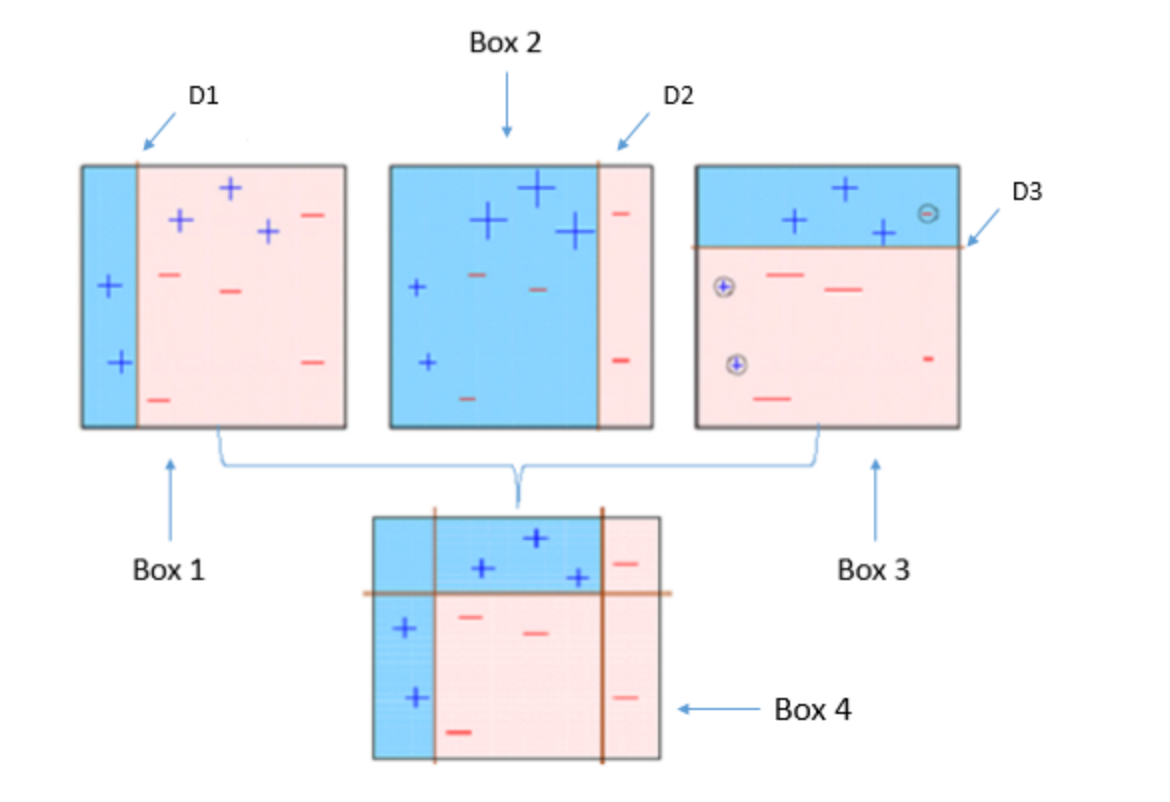
\includegraphics[scale=0.5]{figures/adaboost.png}
              \\
              \tiny
              Source: \url{https://www.analyticsvidhya.com/blog/2015/11/quick-introduction-boosting-algorithms-machine-learning/}
 \end{figure}

\end{frame}
%----------------------------------------------------------------------%
\begin{frame}[fragile]
\frametitle{Boosting: Motivation}

\begin{itemize}


\item The idea of ensemble learning is to build a prediction model by combining the strengths of a collection of simpler base models.
\medskip
\item  Bagging and random forests form committee of trees, where each cast a vote for the predicted class. 
\medskip
\item Boosting is like as a committee method as well, although unlike random forests, the committee of weak learners evolves over time, and the members cast a weighted vote.


\end{itemize}

\end{frame}
 %----------------------------------------------------------------------%
\subsection{Boosting Trees}
 %----------------------------------------------------------------------%
\begin{frame}[fragile]
\frametitle{Boosting Trees}

\begin{itemize}


\item The goal here is to solve something which looks like
\begin{align}
f^\star=\underset{f\in\mathcal{F}}{\text{argmin}}\left\lbrace \sum_{i=1}^n L(y_i,f(\mathbf{x}_i)) \right\rbrace
\end{align}


\item for some loss function $L$, and for some set of predictors $\mathcal{F}$. 
\medskip
\item This is an optimization problem. 
\medskip
\item Note that here in a function space, so we are solving for a function not a point.
\end{itemize}


\end{frame}
 %----------------------------------------------------------------------%
\begin{frame}[fragile]
\frametitle{Boosting Trees}

\begin{itemize}
\item From from a numerical perspective, optimization is solve using gradient descent (this is why this technique is also called gradient boosting). 
\end{itemize}

\begin{figure}[H] \centering
            \captionsetup{justification=centering}
              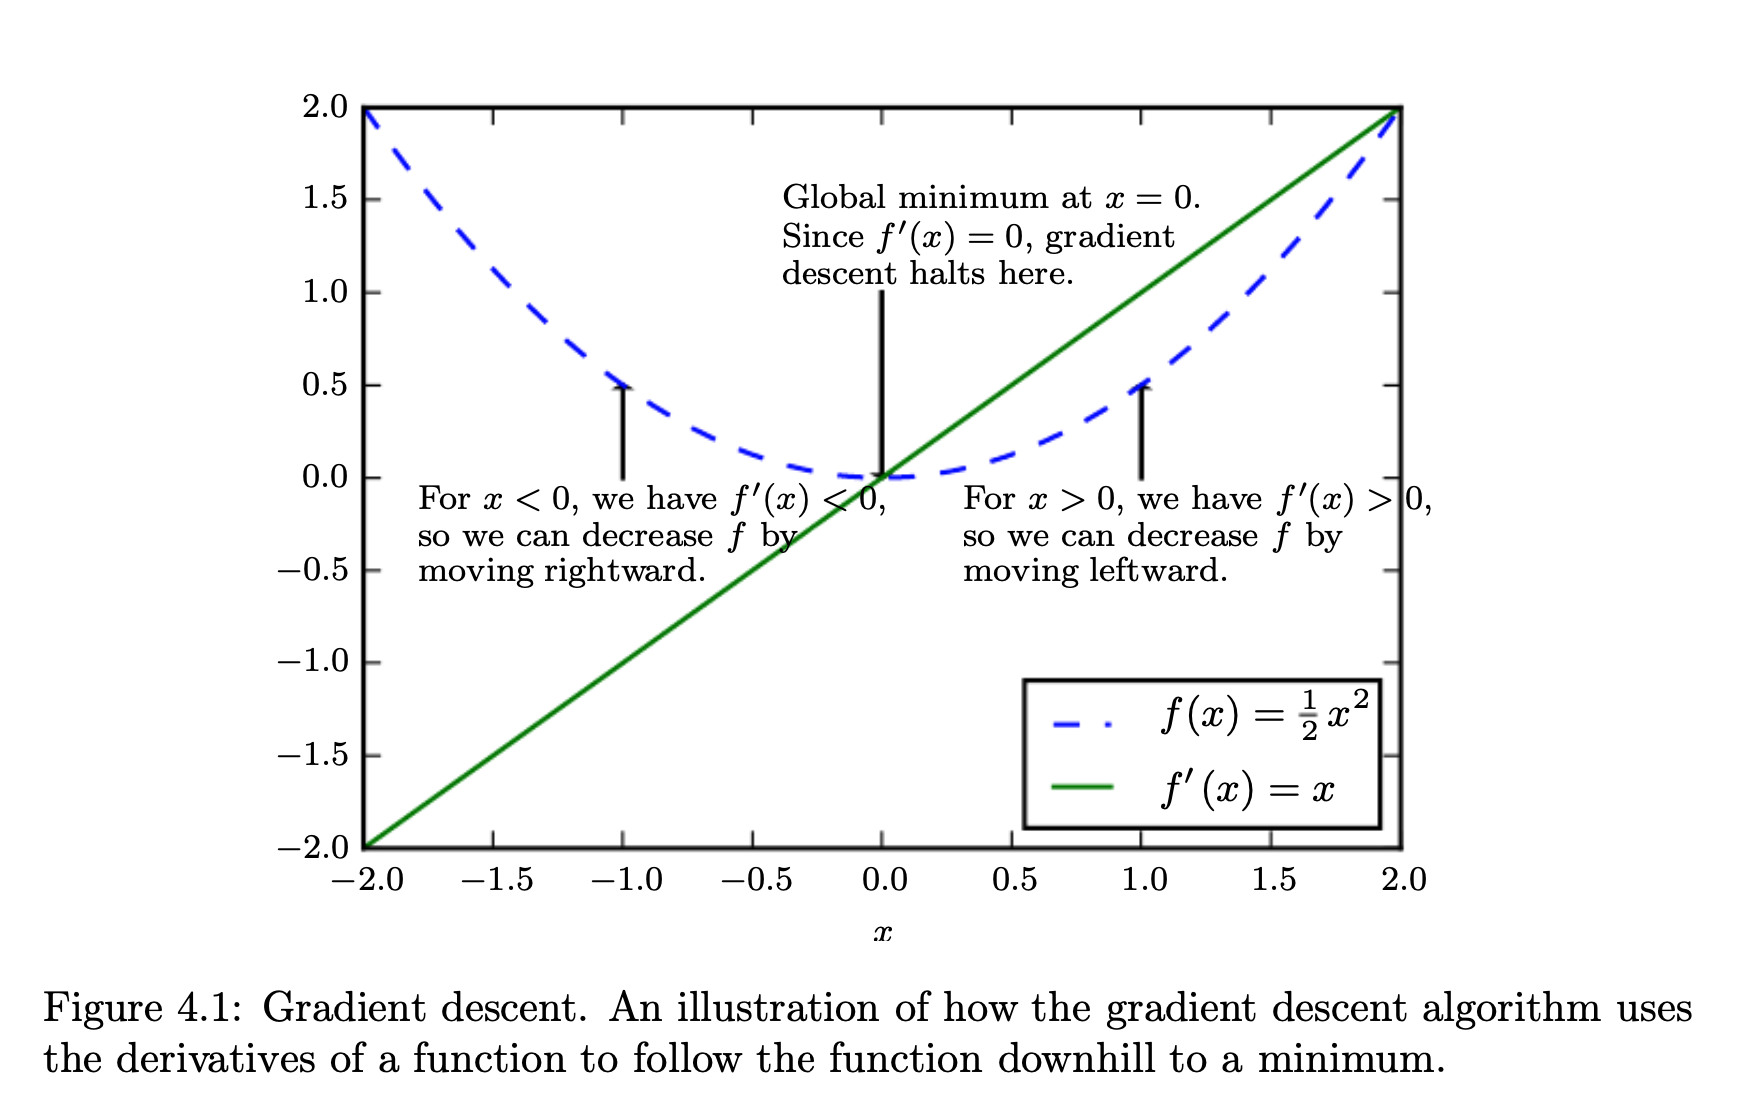
\includegraphics[scale=0.3]{figures/gradient_descent}
              \\
              \tiny
              Source: Goodfellow, I., Bengio, Y., Courville, A., \& Bengio, Y. (2016). Deep learning. Cambridge: MIT press.
 \end{figure}


\end{frame}
%----------------------------------------------------------------------%
%----------------------------------------------------------------------%
\begin{frame}[fragile]
\frametitle{Boosting Trees}

\begin{itemize}


\item Again, the optimum is not some some real value $x^\star$, but some function $m^\star$. 
\item Thus, here we will have something like

\begin{align}
f^{m}=f^{m-1}+\underset{h\in H}{argmin}\sum_{i=1}^n(y_i,f^{m-1}(x_i)+h(x_i))
\end{align}

\item If we consider using mean squared error (MSE) as our loss function, the objective becomes

\begin{align}
\sum_{i=1}^N (f^m_i-\hat{f}_i^{m-1} + \phi_m(x_i))^2
\end{align}

\item  For other losses of interest (for example, logistic loss), it is not so easy to get such a nice form.
\end{itemize}
 \end{frame}
%----------------------------------------------------------------------%
\begin{frame}[fragile]
\frametitle{Boosting Trees: Algorithm explained}

\begin{itemize}
\item  So in the general case, we take the Taylor expansion of the loss function:

\begin{align}
obj^m &= \sum_{i=1}^N \left[ L(f_i,\hat{f}_i^{(m)}) + g_{im} \phi_m(x_i) \right]
\end{align}

where 

\begin{align}
        g_{im}=-\left.\frac{\partial L(f_i,\phi(\mathbf{x}_i))}{\partial \phi(\mathbf{x}_i)}\right\vert_{\phi(\mathbf{x}_i)=\phi^{(m-1)}(\mathbf{x}_i)}
  \end{align}

\item The goal is to fit a model so that $g_{im}=\phi^*(x_i)$
\item when we have that optimal function, set $f^{m}=f^{m-1}+\phi^*(x_i)$
\end{itemize}
 \end{frame}
%----------------------------------------------------------------------%
\begin{frame}[fragile]
\frametitle{Boosting Trees: Algorithm explained}


\begin{itemize}
\item After we remove all the constants, the specific objective at step $m$ becomes


\begin{align}
obj^m &= \sum_{i=1}^N \left[ g_{im} \phi_m(x_i) \right]
\end{align}

\item This becomes our optimization goal for the new tree. One important advantage of this definition is that the value of the objective function only depends on $g_i$ 
\end{itemize}
 \end{frame}


%----------------------------------------------------------------------%
\begin{frame}[fragile]
\frametitle{Boosting Trees}
\framesubtitle{Implementations of Gradient Boosting}

\begin{itemize}
\item Gradient Tree Boosting Algorithm
\medskip
\begin{enumerate}
\item Initialize $f_0(x)=0$ and $g_i=y_i$ for all $i$
\medskip
\item for $m=1$ to $M$:
  \begin{enumerate}
      \item For $i=1,2,\dots N$ compute $g_{im}$
      \medskip
      \item Fit a regression tree to the targets $g_{im}$ giving terminal regions $R_{jm}$ $j=1,2,\dots J_m$
      \medskip
      \item For $j=1,2,\dots,J_m$ compute
      \begin{align}
       c_{jm} =\underset{c}{argmin} \sum_{x_i\in R_{jm} } L(y_i,f_{m-1}(x_i)+c)
      \end{align}
      \medskip
      \item Update $f_m (x)=f_{(m-1)}(x) + \sum_{j=1}^{J_m} c_{jm} I(x \in R_{jm})$
      \medskip
  \end{enumerate}
  \item Output $\hat{f}(x)=\sum^M_i f_m(x)$
\end{enumerate}


\end{itemize}

\end{frame}


%----------------------------------------------------------------------%
\begin{frame}[fragile]
\frametitle{Boosting Trees: Algorithm explained}

\begin{itemize}
\item Learning tree structure is much harder than traditional optimization problem where you can simply take the gradient. 
\medskip
\item It is intractable to learn all the trees at once.
\medskip
\item Instead, we use an additive strategy
\end{itemize}

 \end{frame}
%----------------------------------------------------------------------%
\begin{frame}[fragile]
\frametitle{Boosting Trees: Algorithm explained}

\begin{itemize} 
\item Instead, we use an additive strategy: fix what we have learned, and add one new tree at a time. We write the prediction value at step m as $\hat{y}_i^{m}$. 
\begin{align}
\hat{y}_i^{0} &=0 \\ \nonumber
\hat{y}_i^{1} &= \hat{y}_i^{0} + f_1(x_i) \\ \nonumber
\dots \\ \nonumber
\hat{y}_i^{M} &= \sum_{m=1}^M f_m(x_i) = \hat{y}_i^{m-1} + f_m(x_i) \\ \nonumber
\end{align}

\item Which tree do we want at each step?  Add the one that optimizes our objective.

\begin{align}
obj^m &= \sum_{i=1}^N L(y_i,\hat{y}_i^{(m)}) = \sum_{i=1}^N \left[ g_{im} \phi_m(x_i) \right]
\end{align}
\end{itemize}


 \end{frame}

%----------------------------------------------------------------------%
\begin{frame}[fragile]
\frametitle{Boosting Trees: Example}
\begin{figure}[H] \centering
            \captionsetup{justification=centering}
              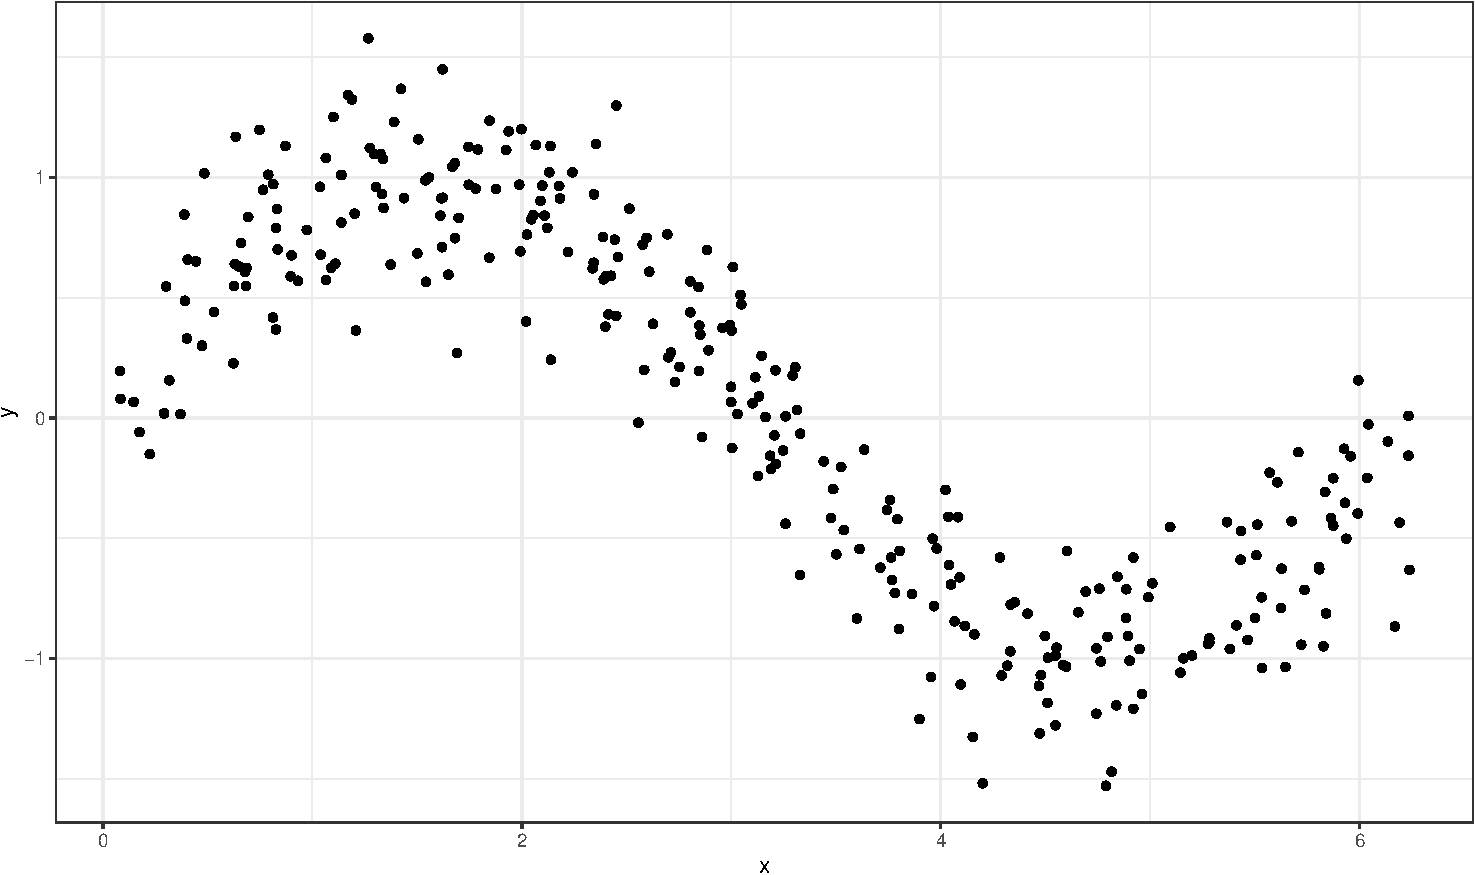
\includegraphics[scale=0.5]{figures/unnamed-chunk-3-1.pdf}
 \end{figure}


 \end{frame}
%----------------------------------------------------------------------%
\begin{frame}[fragile, noframenumbering]
\frametitle{Boosting Trees: Example}

\begin{itemize}
\item Algorithm:
\end{itemize}

\begin{Shaded}
\begin{Highlighting}[]
\NormalTok{M\textless{}{-}}\DecValTok{2}
\end{Highlighting}
\end{Shaded}

\begin{figure}[H] \centering
            \captionsetup{justification=centering}
              
\includegraphics[scale=0.5]{figures/unnamed-chunk-5-1.pdf}
 \end{figure}

 \end{frame}
%----------------------------------------------------------------------%
\begin{frame}[fragile, noframenumbering]
\frametitle{Boosting Trees: Example}

\begin{Shaded}
\begin{Highlighting}[]
\NormalTok{M\textless{}{-}}\DecValTok{10}
\end{Highlighting}
\end{Shaded}

\begin{figure}[H] \centering
            \captionsetup{justification=centering}
              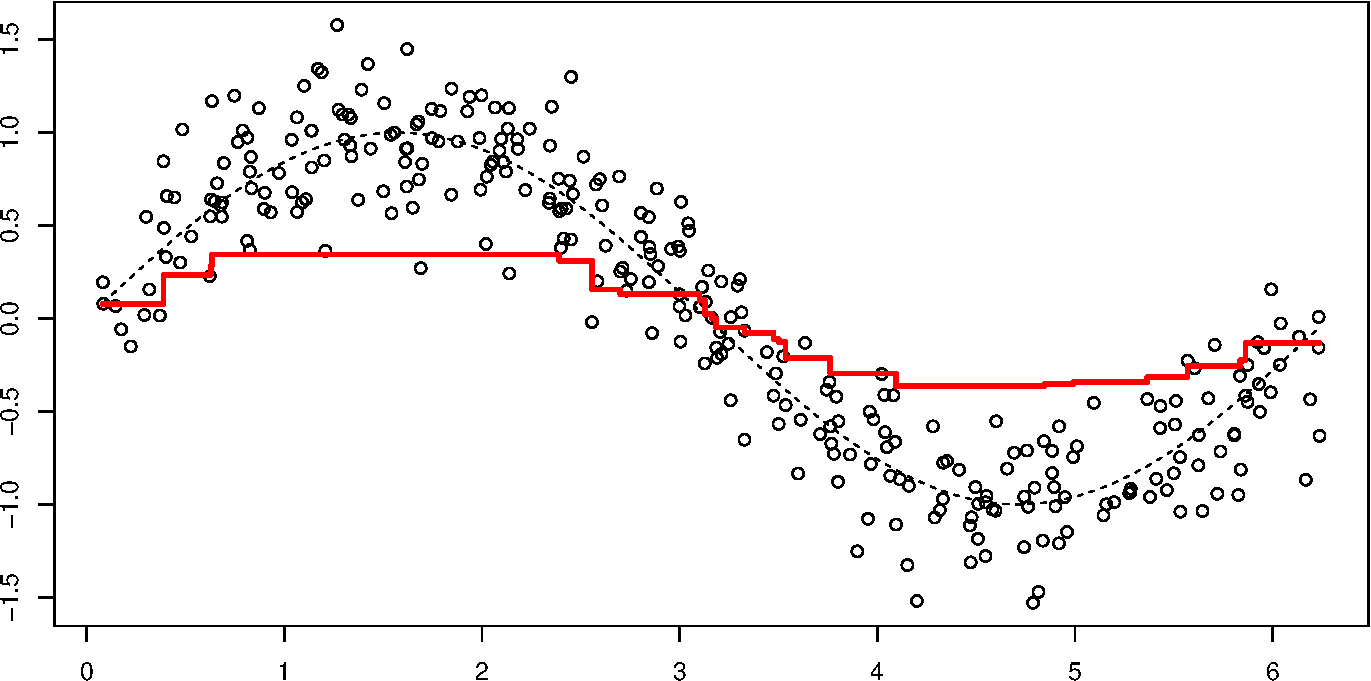
\includegraphics[scale=0.5]{figures/unnamed-chunk-6-1.pdf}
 \end{figure}
 \end{frame}
%----------------------------------------------------------------------%
\begin{frame}[fragile, noframenumbering]
\frametitle{Boosting Trees: Example}

\begin{Shaded}
\begin{Highlighting}[]
\NormalTok{M\textless{}{-}}\DecValTok{100}
\end{Highlighting}
\end{Shaded}

\begin{figure}[H] \centering
            \captionsetup{justification=centering}
              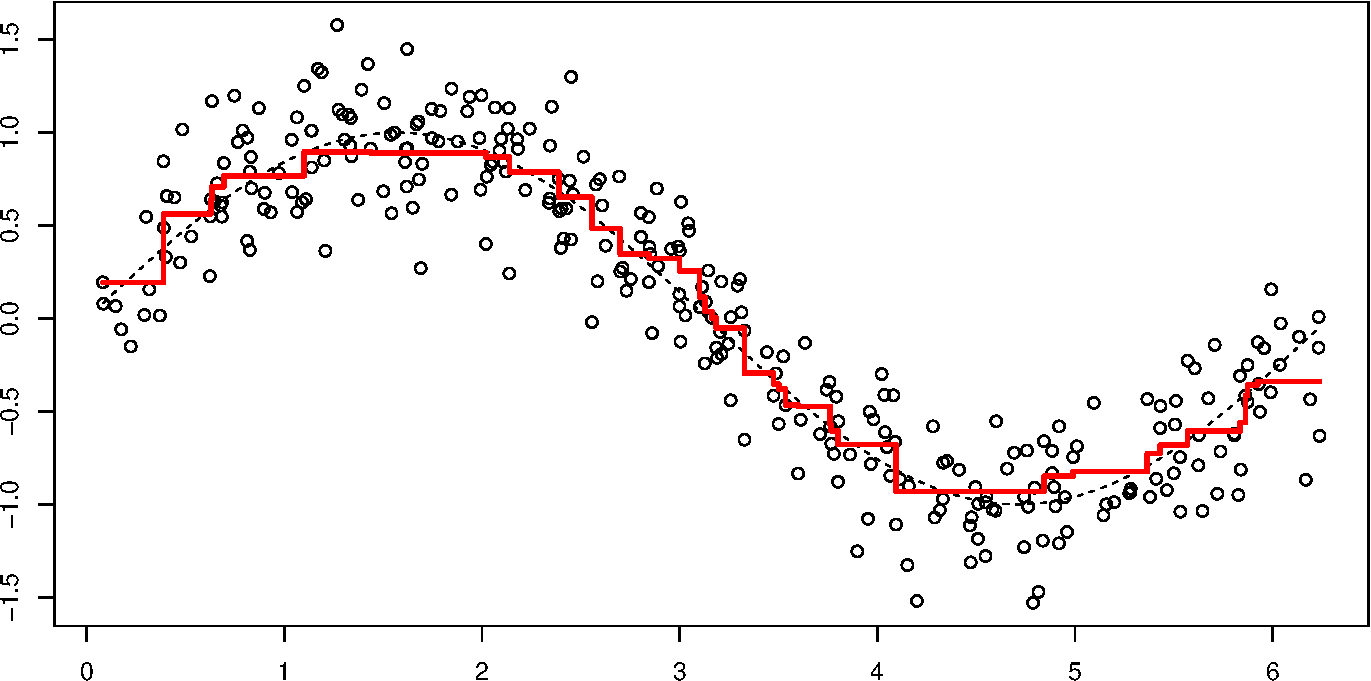
\includegraphics[scale=0.5]{figures/unnamed-chunk-7-1.pdf}
 \end{figure}

 \end{frame}
%----------------------------------------------------------------------%
\begin{frame}[fragile, noframenumbering]
\frametitle{Boosting Trees: Example}

\begin{Shaded}
\begin{Highlighting}[]
\NormalTok{M\textless{}{-}}\DecValTok{300}

\end{Highlighting}
\end{Shaded}

\begin{figure}[H] \centering
            \captionsetup{justification=centering}
              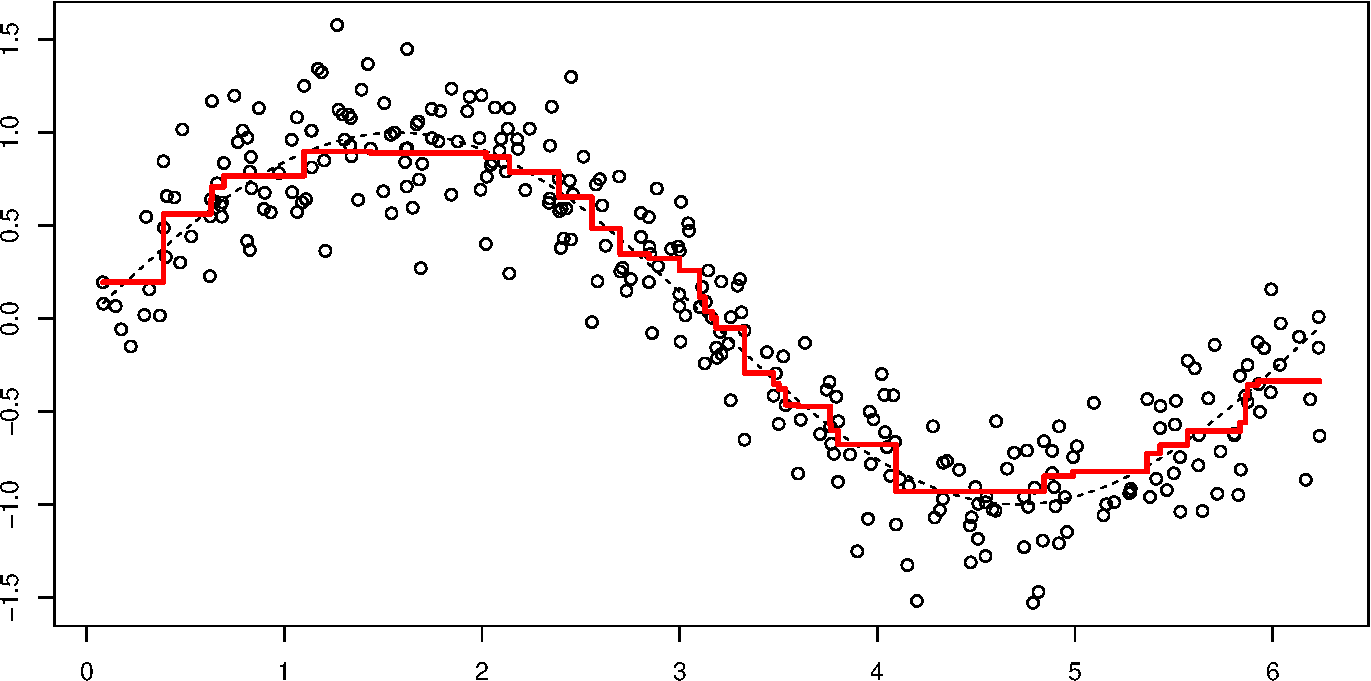
\includegraphics[scale=0.5]{figures/unnamed-chunk-8-1.pdf}
 \end{figure}

 \end{frame}
%----------------------------------------------------------------------%
\begin{frame}[fragile, noframenumbering]
\frametitle{Boosting Trees: Example}

\begin{itemize}
\item Simple tree (blue), boosted tree (red)
\end{itemize}

\begin{figure}[H] \centering
            \captionsetup{justification=centering}
              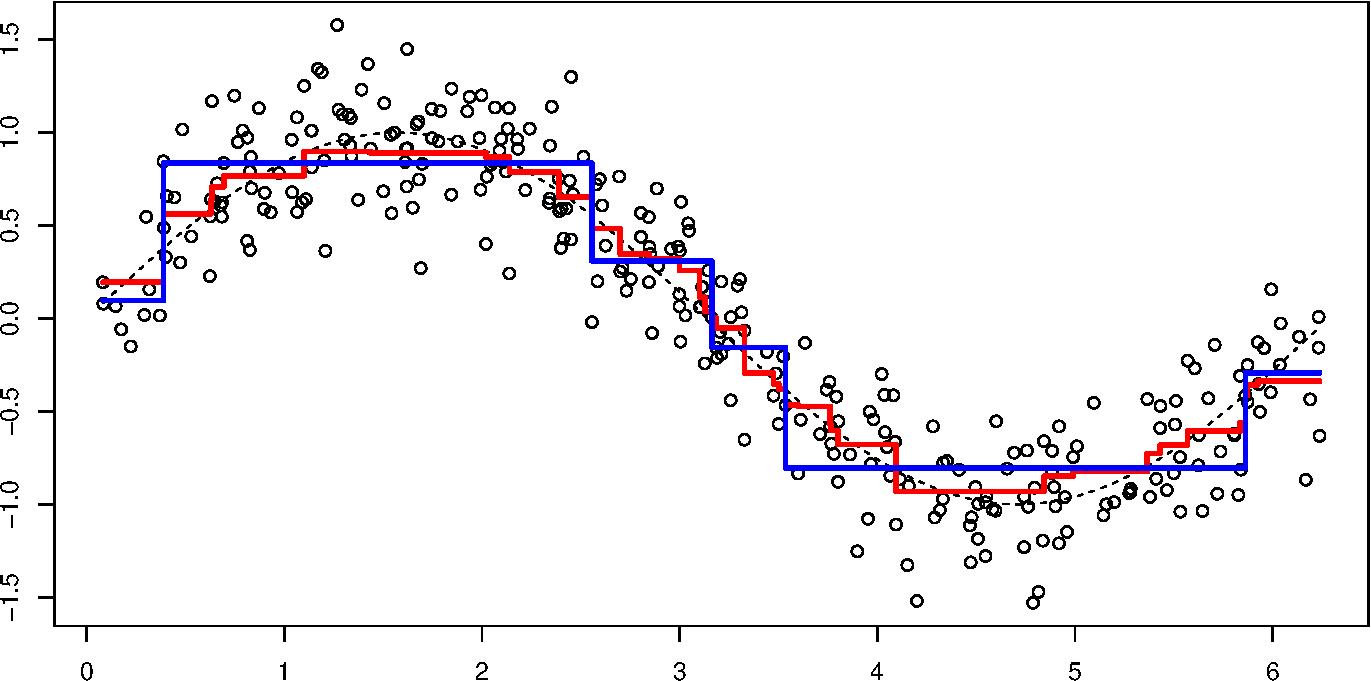
\includegraphics[scale=0.5]{figures/unnamed-chunk-9-1.pdf}
 \end{figure}

 \end{frame}

%----------------------------------------------------------------------%
\begin{frame}[fragile]
\frametitle{Boosting Trees: Parameters}

\begin{itemize}

\item How many iterations (M)?
\begin{itemize}
\medskip

\item Each iteration usually reduces the training risk $L(.)$, so that for M large enough this risk can be made arbitrarily small.
\medskip
\item  However, fitting the training data too well can lead to overfitting, which degrades the risk on future predictions. 

\medskip
\item We use cross-validation
\end{itemize}
\end{itemize}
\end{frame}

%----------------------------------------------------------------------%
\begin{frame}[fragile]
\frametitle{Boosting Trees: Parameters}
\begin{itemize}
\item Can we have shrinkage?
\begin{itemize}
  \item The simplest implementation of shrinkage in the context of boosting is to scale the contribution of each tree by a factor $\nu \in (0,1)$ when it is added to the current approximation. That is, we replace step 
  \begin{align}
   \hat{y}_m (x)=f_{(m-1)}(x) + \nu \phi_m(x_i)
  \end{align}
  \item Empirically it has been found  that smaller values of $\nu$ favor better test error, and require correspondingly larger values of $M$. 
  \item the best strategy appears to be to set $\nu$ to be very small ($\nu < 0.1$)
  \item This yields dramatic improvements (over no shrinkage $\nu$ = 1) 
\end{itemize} 

\end{itemize}

\end{frame}

%----------------------------------------------------------------------%
\begin{frame}[fragile]
\frametitle{Boosting Trees: Parameters}
\begin{itemize}
\item How deep should my trees be?
\begin{itemize}
  \item Often using stumps works well (Tree with a single split)
  \medskip
  \item In this case, the boosted ensemble is fitting an additive model, since each term involves only a single variable.
\medskip
\end{itemize}

\item Can I subsample? Yes, rows and columns
\medskip
\begin{itemize}
\item With stochastic gradient boosting, at each iteration we sample a fraction $\eta$ of the training observations (without replacement), and grow the next tree using that subsample. 
\medskip
\item Reduces the computing time by the same fraction $\eta$, and some cases improves prediction
\medskip
\item Same for columns and breaks high correlation (like forests)
\end{itemize}
\end{itemize}
\end{frame}
%----------------------------------------------------------------------%
\section{XGBoost}
%----------------------------------------------------------------------%
\begin{frame}[fragile]
\frametitle{XGBoost: Motivation}

\begin{itemize}


\item Now that you understand decision trees and gradient boosting,  XGBoost is a walk in the park
\item It is a gradient boosting algorithm that uses decision trees 
\item Beyond that, its implementation was specifically engineered for optimal performance and speed.



\item Why talk about XGBoost?
\begin{itemize}
\scriptsize

 \item Among the 29 challenge winning solutions published in Kaggle's blog during 2015, 17 solutions used XGBoost.  
 \item Among these solutions,  eight  solely  used  XGBoost  to  train  the  model, while most others combined XGBoost with neural nets in ensembles. (The second most popular method, deep  neural  nets,  was  used  in  11  solutions) 
 \item   The  success of the system was also witnessed in 2015 Data Mining and Knowledge Discovery competition organized by ACM (KDD Cup) , where XGBoost  was  used  by  every  winning  team  in  the  top-10. 
 \item Historically, XGBoost has performed quite well for structured, tabular data. But, if you are dealing with non-structured data such as images, neural networks are usually a better option (more on this later)
\end{itemize}
 \end{itemize}
\end{frame}




%----------------------------------------------------------------------%
\begin{frame}[fragile]
\frametitle{XGBoost is a Boosting Tree }

\begin{itemize}


\item Which tree do we want at each step? 
\item Add the one that optimizes our objective.

\begin{align}
\mathcal{L} &= \sum_{i=1}^N L(y_i,\hat{y}_i) + \sum_{k=1}^m \Omega(f_k)
\end{align}

\item  $L(.)$ is a differentiable convex loss function that measures the difference between the prediction $\hat{y}_i$ and the target $y_i$. 
\item  The second term $\Omega(f)$ penalizes the complexity of the model, where


\begin{align}
\Omega(f)=\gamma T + \frac{1}{2}\lambda ||\omega||_2
\end{align}


\end{itemize}
 \end{frame}
%----------------------------------------------------------------------%
\begin{frame}[fragile]
\frametitle{XGBoost is a Boosting Tree }

\begin{itemize}
\item The function above cannot be optimized using traditional optimization methods
\item Let $\mathcal{L}^m$ be the loss at step $m$, then $\hat{y}_i^m$ is the prediction of row $i$ at the $m$ iteration
\item We need to add $f_m$ to minimize the following objective
  \begin{align}
\mathcal{L}^m=\sum_{i=1}^N (y_i-\hat{y}_i^{m-1} + f_m(x_i))^2  +  \Omega(f_t)
\end{align}

\item  So in the general case, we take a second order  Taylor expansion of the loss function:

\begin{align}
\mathcal{L}^m &= \sum_{i=1}^N \left[ L(y_i,\hat{y}_i^{(m-1)}) + g_{im} f_m(x_i) + \frac{1}{2}h_i f^2_m(x_i) \right] +  \Omega(f_t)
\end{align}

where  $g_{im} = \frac{\partial L(y_i,\hat{y}_i^{(m-1)})}{\partial f^{(m-1)}(\mathbf{x}_i)}$ and $h_{im} = \frac{\partial^2 L(y_i,\hat{y}_i^{(m-1)})}{\partial (f^{(m-1)}(\mathbf{x}_i))^2}$
  \end{itemize}
 \end{frame}
%----------------------------------------------------------------------%
\begin{frame}[fragile]
\frametitle{XGBoost is a Boosting Tree }

\begin{itemize}


\item After we remove all the constants, the specific objective at step m becomes
\medskip

\begin{align}
\mathcal{L}^m &= \sum_{i=1}^N \left[ g_{im} f_m(x_i) + \frac{1}{2}h_i f^2_m(x_i) \right] +  \Omega(f_t)
\end{align}
\medskip
\item This becomes our optimization goal for the new tree. 
\medskip
\item One important advantage of this definition is that the value of the objective function only depends on $g_{im}$ and $h_{im}$ 


\end{itemize}



 \end{frame}

%----------------------------------------------------------------------%
\begin{frame}[fragile]
\frametitle{XGBoost Model Complexity}

\begin{itemize}
\item Let's talk about the  regularization term 
\item We need to define the complexity of the tree $\Omega(f)$.
\item But us first refine the definition of the tree $f(x)$ as

 
\begin{align}
f_t(x) = w_{q(x)}, w \in R^T, q:R^d\rightarrow \{1,2,\cdots,T\} .
\end{align}


\item Here $w$ is the vector of predictions on leaves, $q$ is a function assigning each data point to the corresponding leaf, and $T$ is the number of leaves. 

\end{itemize}

 \end{frame}

%----------------------------------------------------------------------%
\begin{frame}[fragile]
\frametitle{XGBoost Model Complexity}

\begin{itemize}
\item In XGBoost, they define the complexity as
\begin{align}
\Omega(f) = \gamma T + \frac{1}{2}\lambda \sum_{j=1}^T w_j^2
\end{align}




\item The regularization is one part most tree packages treat less carefully, or simply ignore. 
\medskip 
\item This was because the traditional treatment of tree learning only emphasized improving impurity, while the complexity control was left to heuristics.
\medskip 
\item  By defining it formally, we can get a better idea of what we are learning and obtain models that perform well in the wild.

\end{itemize}
 \end{frame}

%----------------------------------------------------------------------%
\begin{frame}[fragile]
\frametitle{XGBoost Model Complexity}

\begin{itemize}
\item With the aboe notation we can re writ the objective funtion as 


\begin{align}
\mathcal{L}^{(t)} &\approx \sum_{i=1}^n [g_i w_{q(x_i)} + \frac{1}{2} h_i w_{q(x_i)}^2] + \gamma T + \frac{1}{2}\lambda \sum_{j=1}^T w_j^2\\
&= \sum^T_{j=1} [(\sum_{i\in I_j} g_i) w_j + \frac{1}{2} (\sum_{i\in I_j} h_i + \lambda) w_j^2 ] + \gamma T\
\end{align}

\item where $I_j={i|q(x_i)=j}$ set of indicators that assign to the $j-th$ leaf.
\item Note the following in the second line, we changed the index of the summation because all the data points on the smae leaf get the same score.
\item Defining $G_j = \sum_{i\in I_j} g_i$ and $H_j = \sum_{i\in I_j} h_i$

\begin{align}
\mathcal{L}^{(t)} = \sum^T_{j=1} [G_jw_j + \frac{1}{2} (H_j+\lambda) w_j^2] +\gamma T
\end{align}

\end{itemize}

\end{frame}

%----------------------------------------------------------------------%
\begin{frame}[fragile]
\frametitle{XGBoost Model Complexity}

\begin{itemize}
\item In the above equation, $w_j$ are independent with respect to each other, 
\item the form $G_jw_j+\frac{1}{2}(H_j+\lambda)w_j^2$  is quadratic 
\item then the best $w_j$ for a given structure tree structure $q(x)$ get is:


\begin{align}
w_j^\ast &= -\frac{G_j}{H_j+\lambda}\\
\end{align}


\item and the best objective reduction we can get

\begin{align}
\mathcal{L}^\ast &= -\frac{1}{2} \sum_{j=1}^T \frac{G_j^2}{H_j+\lambda} + \gamma T
\end{align}

\end{itemize}



\end{frame}
%----------------------------------------------------------------------%
\begin{frame}[fragile]
\frametitle{XGBoost Model Complexity: Example}
  \begin{figure}[H] \centering
            \captionsetup{justification=centering}
              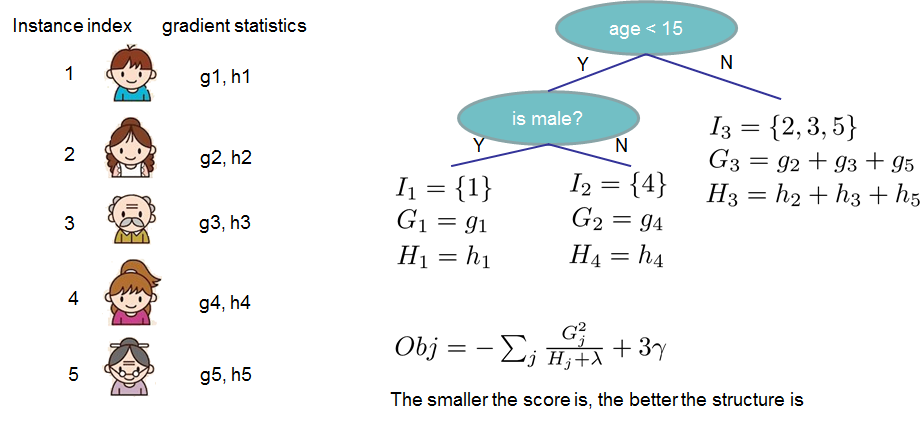
\includegraphics[scale=0.6]{figures/struct_score}
              \\
              \tiny
              \url{source: https://xgboost.readthedocs.io/en/latest/tutorials/model.html}
 \end{figure}

 \end{frame}
%----------------------------------------------------------------------%
\begin{frame}[fragile]
\frametitle{Learn the tree structure}

\begin{itemize}
\item Now that we have a way to measure how good a tree is, 
\medskip
\item Ideally we would enumerate all possible trees and pick the best one. 
\medskip
\item In practice this is intractable, so we will try to optimize one level of the tree at a time. 
\medskip
\item Specifically we try to split a leaf into two leaves, and the score it gains is
\end{itemize}
\begin{align}
Gain = \frac{1}{2} \left[\frac{G_L^2}{H_L+\lambda}+\frac{G_R^2}{H_R+\lambda}-\frac{(G_L+G_R)^2}{H_L+H_R+\lambda}\right] - \gamma
\end{align}

 \end{frame}
%----------------------------------------------------------------------%
\begin{frame}[fragile]
\frametitle{Learn the tree structure}

\begin{itemize}
  \item This formula can be decomposed as 
  \medskip
\begin{enumerate}
\item  the score on the new left leaf 
\medskip
\item the score on the new right leaf 
\medskip
\item the score on the original leaf 
\medskip
\item  regularization on the additional leaf. 
\end{enumerate}
\item We can see an important fact here: if the gain is smaller than $\gamma$ , we would do better not to add that branch. This is exactly the pruning techniques in tree based models

\item For real valued data, we usually want to search for an optimal split. To efficiently do so, we place all the instances in sorted order


\end{itemize}


 \end{frame}
%----------------------------------------------------------------------%
\begin{frame}[fragile]
\frametitle{Learn the tree structure}

\begin{itemize}

\item A left to right scan is sufficient to calculate the structure score of all possible split solutions, and we can find the best split efficiently
\end{itemize}

  \begin{figure}[H] \centering
            \captionsetup{justification=centering}
              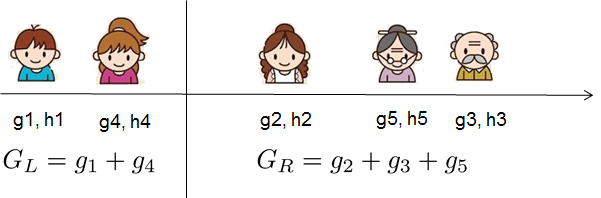
\includegraphics[scale=0.6]{figures/tree_structure}
              \\
              \tiny
              \url{source: https://xgboost.readthedocs.io/en/latest/tutorials/model.html}
 \end{figure}
 
\end{frame}




%----------------------------------------------------------------------%
%----------------------------------------------------------------------%
\section{Review
 \& Next Steps}
%----------------------------------------------------------------------%
\begin{frame}
\frametitle{Review \& Next Steps}
  
\begin{itemize} 
    \item Gradient Based Optimization
    \medskip
    \item Boosting Trees
    \begin{itemize}
      \item How it works
    \end{itemize}
    \item XGBoost
    \begin{itemize}
      \item How it works
    \end{itemize}
    \item Preview next class: superlearners and text
    \medskip  
    \item Questions? Questions about software? 

\end{itemize}
\end{frame}
%----------------------------------------------------------------------%
\section{Further Readings}
%----------------------------------------------------------------------%
\begin{frame}
\frametitle{Further Readings}

\begin{itemize}

  \item Charpentier, Arthur (2018). Classification from scratch, boosting. \url{https://freakonometrics.hypotheses.org/tag/xgboost}
  \medskip
  \item Chen, T., \& Guestrin, C. (2016, August). Xgboost: A scalable tree boosting system. In Proceedings of the 22nd acm sigkdd international conference on knowledge discovery and data mining (pp. 785-794).
  \medskip
  \item Friedman, J., Hastie, T., \& Tibshirani, R. (2001). The elements of statistical learning (Vol. 1, No. 10). New York: Springer series in statistics.
  \medskip
  \item Goodfellow, I., Bengio, Y., Courville, A., \& Bengio, Y. (2016). Deep learning. Cambridge: MIT press.

  
\end{itemize}

\end{frame}


%----------------------------------------------------------------------%
%----------------------------------------------------------------------%
\appendix
\newcounter{finalframe}
\setcounter{finalframe}{\value{framenumber}}
\normalsize


%----------------------------------------------------------------------%
\section{XGBoost: Demo}
%----------------------------------------------------------------------%
\begin{frame}[fragile]
\frametitle{XGBoost: Demo}



\begin{Shaded}
\begin{Highlighting}[]
\CommentTok{\#Load the required packages}
\KeywordTok{library}\NormalTok{(}\StringTok{"McSpatial"}\NormalTok{) }\CommentTok{\#loads the package}
\KeywordTok{library}\NormalTok{(}\StringTok{"dplyr"}\NormalTok{) }\CommentTok{\#for data wrangling}
\KeywordTok{library}\NormalTok{(}\StringTok{"caret"}\NormalTok{)}

\KeywordTok{data}\NormalTok{(matchdata) }\CommentTok{\#loads the data set}
\KeywordTok{set.seed}\NormalTok{(}\DecValTok{123}\NormalTok{) }\CommentTok{\#set the seed for replication purposes}
\end{Highlighting}
\end{Shaded}

\begin{Shaded}
\begin{Highlighting}[]
\CommentTok{\#linear regression}
\NormalTok{model\_lm\textless{}{-}}\KeywordTok{train}\NormalTok{(lnprice}\OperatorTok{\textasciitilde{}}\NormalTok{.}\OperatorTok{+}\NormalTok{.}\OperatorTok{:}\NormalTok{latitude}\OperatorTok{+}\NormalTok{.}\OperatorTok{:}\NormalTok{longitude}\OperatorTok{+}\NormalTok{.}\OperatorTok{:}\NormalTok{latitude}\OperatorTok{:}\NormalTok{longitude,  }
                     \DataTypeTok{data =}\NormalTok{ matchdata,}
                     \DataTypeTok{trControl =} \KeywordTok{trainControl}\NormalTok{(}\DataTypeTok{method =} \StringTok{"cv"}\NormalTok{, }\DataTypeTok{number =} \DecValTok{5}\NormalTok{), }
                     \DataTypeTok{method =} \StringTok{"lm"}\NormalTok{)    }
\end{Highlighting}
\end{Shaded}

\end{frame}
%----------------------------------------------------------------------%
\begin{frame}[fragile]
\frametitle{XGBoost: Demo}


\begin{Shaded}
\begin{Highlighting}[]
\NormalTok{model\_lm}
\end{Highlighting}
\end{Shaded}

\begin{tiny}
\begin{verbatim}
## Linear Regression 
## 
## 3204 samples
##   17 predictor
## 
## No pre-processing
## Resampling: Cross-Validated (5 fold) 
## Summary of sample sizes: 2562, 2564, 2561, 2564, 2565 
## Resampling results:
## 
##   RMSE       Rsquared   MAE      
##   0.2058519  0.8472526  0.1442374
## 
## Tuning parameter 'intercept' was held constant at a value of TRUE
\end{verbatim}
\end{tiny}
\end{frame}
%----------------------------------------------------------------------%
\begin{frame}[fragile]
\frametitle{XGBoost: Demo}
\begin{itemize}
\item From \texttt{Caret's} manual

\item eXtreme Gradient Boosting
\medskip
\begin{itemize}
\item method = `xgbTree'
\medskip
\item Type: Regression, Classification
\medskip
\item Tuning parameters:

  
  \begin{verbatim}
  nrounds (# Boosting Iterations)
  max_depth (Max Tree Depth)
  eta (Shrinkage)
  gamma (Minimum Loss Reduction)
  colsample_bytree (Subsample Ratio of Columns)
  min_child_weight (Minimum Sum of Instance Weight)
  subsample (Subsample Percentage)
  \end{verbatim}



  \item Required packages: xgboost, plyr
  \medskip
  \item A model-specific variable importance metric is available.
\end{itemize}
\end{itemize}

\end{frame}
%----------------------------------------------------------------------%
\begin{frame}[fragile]
\frametitle{XGBoost: Demo}

\begin{scriptsize}
\begin{Shaded}
\begin{Highlighting}[]

\NormalTok{tune\_grid \textless{}{-}}\StringTok{ }\KeywordTok{expand.grid}\NormalTok{(}
  \DataTypeTok{nrounds =} \KeywordTok{seq}\NormalTok{(}\DataTypeTok{from =} \DecValTok{200}\NormalTok{, }\DataTypeTok{to =} \DecValTok{1000}\NormalTok{, }\DataTypeTok{by =} \DecValTok{50}\NormalTok{),}
  \DataTypeTok{eta =} \KeywordTok{c}\NormalTok{(}\FloatTok{0.025}\NormalTok{, }\FloatTok{0.05}\NormalTok{, }\FloatTok{0.1}\NormalTok{, }\FloatTok{0.3}\NormalTok{),}
  \DataTypeTok{max\_depth =} \KeywordTok{c}\NormalTok{(}\DecValTok{2}\NormalTok{, }\DecValTok{3}\NormalTok{, }\DecValTok{4}\NormalTok{, }\DecValTok{5}\NormalTok{, }\DecValTok{6}\NormalTok{),}
  \DataTypeTok{gamma =} \DecValTok{0}\NormalTok{,}
  \DataTypeTok{colsample\_bytree =} \DecValTok{1}\NormalTok{,}
  \DataTypeTok{min\_child\_weight =} \DecValTok{1}\NormalTok{,}
  \DataTypeTok{subsample =} \DecValTok{1}
\NormalTok{)}

\NormalTok{tune\_control \textless{}{-}}\StringTok{ }\NormalTok{caret}\OperatorTok{::}\KeywordTok{trainControl}\NormalTok{(}
  \DataTypeTok{method =} \StringTok{"cv"}\NormalTok{, }\CommentTok{\# cross{-}validation}
  \DataTypeTok{number =} \DecValTok{3}\NormalTok{, }\CommentTok{\# with n folds }
  \CommentTok{\#index = createFolds(tr\_treated$Id\_clean), \# fix the folds}
  \DataTypeTok{verboseIter =} \OtherTok{FALSE}\NormalTok{, }\CommentTok{\# no training log}
  \DataTypeTok{allowParallel =} \OtherTok{TRUE} \CommentTok{\# FALSE for reproducible results }
\NormalTok{)}
\end{Highlighting}
\end{Shaded}

\end{scriptsize}
\end{frame}
%----------------------------------------------------------------------%
\begin{frame}[fragile]
\frametitle{XGBoost: Demo}

\begin{scriptsize}
\begin{Shaded}
\begin{Highlighting}[]
\NormalTok{input\_x \textless{}{-}}\StringTok{ }\KeywordTok{select}\NormalTok{(matchdata, }\OperatorTok{{-}}\NormalTok{lnprice)}
\NormalTok{input\_x}\OperatorTok{$}\NormalTok{year \textless{}{-}}\KeywordTok{as.factor}\NormalTok{(input\_x}\OperatorTok{$}\NormalTok{year)}
\NormalTok{input\_x}\OperatorTok{$}\NormalTok{carea \textless{}{-}}\KeywordTok{as.factor}\NormalTok{(input\_x}\OperatorTok{$}\NormalTok{carea)}
\KeywordTok{require}\NormalTok{(}\StringTok{"Matrix"}\NormalTok{)}
\end{Highlighting}
\end{Shaded}

\begin{Shaded}
\begin{Highlighting}[]
\NormalTok{input\_x\textless{}{-}}\StringTok{ }\KeywordTok{sparse.model.matrix}\NormalTok{(}\OperatorTok{\textasciitilde{}}\NormalTok{.,}\DataTypeTok{data=}\NormalTok{input\_x)}
\NormalTok{input\_y \textless{}{-}}\StringTok{ }\NormalTok{matchdata}\OperatorTok{$}\NormalTok{lnprice}

\NormalTok{model\_xgb \textless{}{-}}\StringTok{ }\NormalTok{caret}\OperatorTok{::}\KeywordTok{train}\NormalTok{(}
  \DataTypeTok{x =}\NormalTok{ input\_x,}
  \DataTypeTok{y =}\NormalTok{ input\_y,}
  \DataTypeTok{trControl =}\NormalTok{ tune\_control,}
  \DataTypeTok{tuneGrid =}\NormalTok{ tune\_grid,}
  \DataTypeTok{method =} \StringTok{"xgbTree"}\NormalTok{,}
  \DataTypeTok{verbose =} \OtherTok{TRUE}
\NormalTok{)}
\end{Highlighting}
\end{Shaded}


\begin{Shaded}
\begin{Highlighting}[]
\NormalTok{model\_xgb}\OperatorTok{$}\NormalTok{bestTune}
\end{Highlighting}
\end{Shaded}

\begin{verbatim}
##    nrounds max_depth  eta gamma colsample_bytree min_child_weight subsample
## 93     550         2 0.05     0                1                1         1
\end{verbatim}
\end{scriptsize}
\end{frame}
%----------------------------------------------------------------------%
\begin{frame}[fragile]
\frametitle{XGBoost: Demo}



  \begin{figure}[H] \centering
            \captionsetup{justification=centering}
              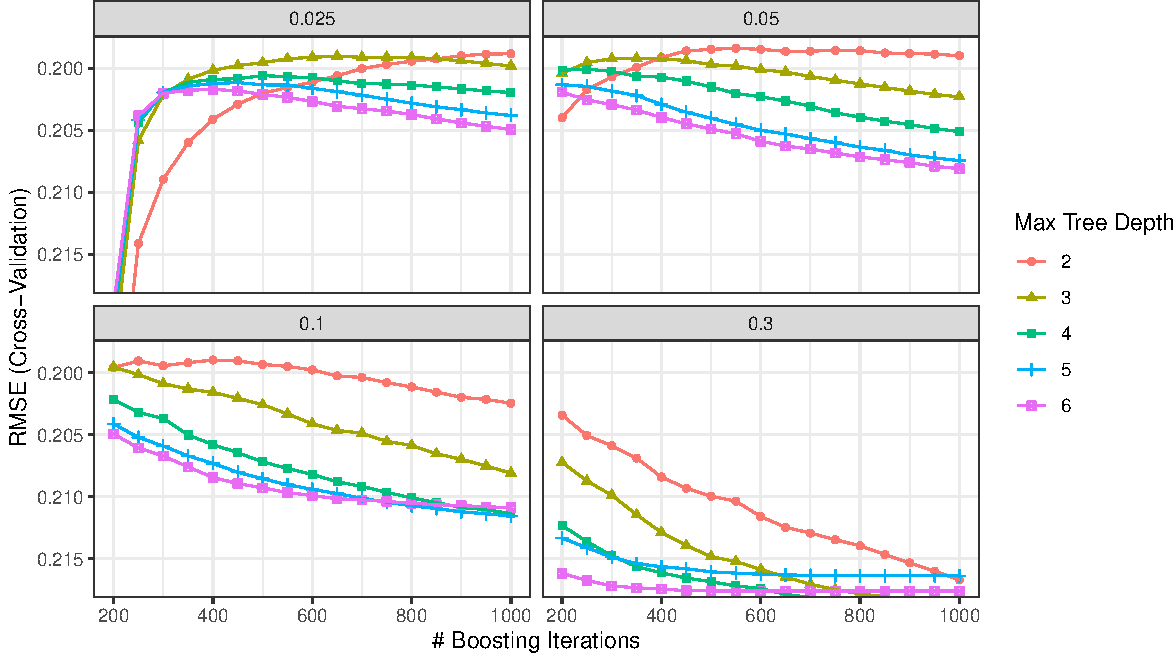
\includegraphics[scale=0.6]{figures/unnamed-chunk-4-1.pdf}
              
 \end{figure}

\end{frame}


%----------------------------------------------------------------------%
%----------------------------------------------------------------------%
\end{document}
%----------------------------------------------------------------------%
%----------------------------------------------------------------------%

